\subsection{Постановка задачи}
  \begin{minipage}{0.6\textwidth}
    \captionof{table}{Геометрия фильтра}
			\begin{tabular}{l l}
				\hline
				\label{geometrytable}
				Диаметр цилиндра, $D$ & $0.205m$ \\
				Диаметр выходной трубы, $D_e$ & $0.5D$ \\
				Высота входного канала, $a$ & $0.5D$ \\
				Ширина входного канала, $b$ & $0.2D$ \\
				Длина выходной трубы, $h_e$ & $0.75D$ \\
				Полная высота фильтра, $H$ & $4.0D$ \\
				Высота цилиндра, $h$ & $1.5D$ \\
				Диаметр нижнего сечения, $B$ & $0.36D$ \\
				Высота пылесборника, $h_d$ & $0.25D$ \\
				Диаметр пылесборника, $D_d$ & $0.75D$ \\
			\end{tabular}
    \end{minipage}
    \hspace{1em}
  \begin{minipage}{0.35\textwidth}
    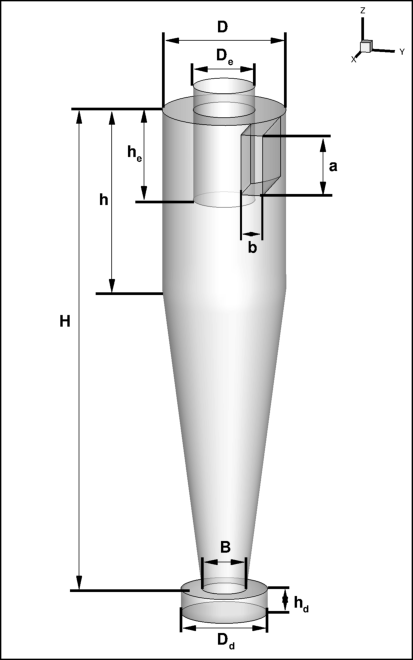
\includegraphics[scale=0.45]{Geometry}
				\captionof{figure}{Схема фильтра}
  \end{minipage}